\documentclass[11pt]{article}
\usepackage[margin=1in]{geometry}
\usepackage{amsmath,amssymb}
\usepackage{graphicx}
\usepackage{booktabs}
\usepackage{microtype}
\usepackage[hidelinks]{hyperref}
\usepackage{xcolor}

\title{\textbf{Clark-Quantize: Data-Free Optimal-Scale Ternary\\
Quantization for Generative Transformers}}
\author{Clark Labs, Inc.}
\date{2026}

\newcommand{\R}{\mathbb{R}}
\newcommand{\sign}{\operatorname{sign}}

\begin{document}
\maketitle

\begin{abstract}
We study post-training quantization of generative transformers to ternary
weights $\{-1,0,+1\}$ at an effective $1.6$--$2.5$ bits per weight, under the
strict constraint of using \emph{no calibration data, no gradients, and no
fine-tuning}. We make a single, sharp observation: at this precision the entire
quality gap is controlled by the per-group \emph{scale}, not by error feedback,
group size, or which layers are protected. The widely used \texttt{absmean} rule
($s=\operatorname{mean}|w|$) is provably suboptimal and, applied to a diffusion
transformer, produces pure noise. Replacing it with the closed-form
mean-squared-error (MSE) optimal ternary scale---which reduces to maximizing
$(\sum_{\text{top-}k}|w|)^2/k$ per group---recovers coherent, prompt-faithful
image generation with $94.6\%$ of the transformer's weights ternary and only six
small layers kept at original precision. On Sana~1.6B the optimal-scale quantizer
improves PSNR-to-baseline from $9.1$\,dB (\texttt{absmean}, indistinguishable from
noise) to $12.0$\,dB at group size $32$, entirely data-free. We then add GPTQ with
a shared incoherence rotation and---our core result---calibrate its Hessian on the
model's \emph{own unconditional prior} (pure Gaussian noise and the null prompt,
which a diffusion model is built to consume), matching prompt-calibration to within
noise ($16.1$ vs $15.9$\,dB) with no external data, gradients, or fine-tuning. This
makes \textbf{data-free, train-free, near-FP16 quantization solved for the attention
and projection layers at $1.7$--$2.1$ bits}. The remaining obstacle is purely
representational: Sana's gated GLU-convolution feed-forward network resists
ultra-low-bit scalar coding. We report a systematic negative result---optimal
ternary, uniform multi-symbol, learned Lloyd--Max codebooks, post-hoc escapes, and
entropy-constrained GPTQ all fail to reach a near-FP16 point below $\sim$2 bits on
this FFN, with a failure mode indicating the missing information is local and
vector-structured rather than scalar. The practical product is a mixed-precision
artifact (ternary attention, $4$-bit FFN) that is data-free, near-FP16, and
$\sim$4--6$\times$ smaller; closing the gap to $8\times$ requires vector or
structural FFN compression. We provide the derivation, an open implementation, and
ablations.
\end{abstract}

\section{Introduction}
Deployment cost---memory footprint, bandwidth, and energy---now dominates the
economics of generative models on edge hardware. Token (or denoising-step)
latency is bound by the cost of streaming weights from memory, so reducing weight
precision attacks the primary bottleneck directly. Ternary weights
$\{-1,0,+1\}$ sit near the practical floor of representation: $\log_2 3\approx
1.585$ bits, plus a small per-group scale overhead.

Most ternary results rely on quantization-aware training or curated calibration
sets. We ask a narrower question: \emph{how good can a purely data-free ternary
post-training quantizer be?} A data-free method needs no held-out corpus, no
forward passes over data, and integrates trivially into any toolchain. Our finding
is that the answer hinges almost entirely on one design choice---the per-group
scale---and that the optimal data-free choice is a closed form that is cheap to
compute and markedly better than the common heuristic.

\section{Method}

\subsection{Group-wise ternary format}
For a weight matrix $W\in\R^{d_\text{out}\times d_\text{in}}$ we partition each row
into contiguous groups of $g$ weights along the input dimension. Each group $G$
stores one FP16 scale $s_G$ and a ternary code $t_i\in\{-1,0,+1\}$ per weight, so
\begin{equation}
  w_i \approx s_G\, t_i,\qquad t_i\in\{-1,0,+1\}.
\end{equation}
Storing $t_i$ in two bits gives $2 + 16/g$ bits/weight (e.g.\ $2.125$ at $g{=}128$,
$2.5$ at $g{=}32$); a tight packing approaches $1.585 + 16/g$. The format is
identical across choices of the quantizer; only $(s_G, t)$ change.

\subsection{The MSE-optimal scale}
Fix a group with weights $w_1,\dots,w_g$. A ternary assignment is determined by a
\emph{support} $S\subseteq\{1,\dots,g\}$ (the indices set to $\pm1$, with sign
$\sign(w_i)$) and a scale $s>0$. The reconstruction error is
\begin{equation}
  \mathcal{E}(S,s) \;=\; \sum_{i\notin S} w_i^2 \;+\; \sum_{i\in S}\bigl(|w_i|-s\bigr)^2 .
\end{equation}
Minimizing over $s$ for fixed $S$ gives the optimal scale
$s^\star = \tfrac{1}{|S|}\sum_{i\in S}|w_i|$, and substituting back,
\begin{equation}
  \min_s \mathcal{E}(S,s)
  \;=\; \sum_{i=1}^{g} w_i^2 \;-\; \frac{\bigl(\sum_{i\in S}|w_i|\bigr)^2}{|S|}.
  \label{eq:residual}
\end{equation}
Since $\sum_i w_i^2$ is constant, minimizing~\eqref{eq:residual} is equivalent to
\begin{equation}
  \max_{S}\; \frac{\bigl(\sum_{i\in S}|w_i|\bigr)^2}{|S|}.
  \label{eq:objective}
\end{equation}
For a fixed cardinality $k=|S|$, the numerator is maximized by the $k$ largest
$|w_i|$; hence the optimal support is a \emph{top-$k$} set and we need only search
$k\in\{1,\dots,g\}$. Sorting $|w|$ once and scanning the prefix sums yields the
global optimum in $O(g\log g)$ per group:
\begin{equation}
  k^\star=\arg\max_k \frac{c_k^2}{k},\quad
  c_k=\sum_{j=1}^{k}|w|_{(j)},\quad
  s^\star=\frac{c_{k^\star}}{k^\star},
\end{equation}
where $|w|_{(1)}\ge|w|_{(2)}\ge\cdots$ are the sorted magnitudes. This is fully
data-free.

\subsection{Why \texttt{absmean} is suboptimal}
The common $1.58$-bit heuristic sets $s=\operatorname{mean}_i|w_i|$ over the whole
group and rounds $t_i=\operatorname{clip}(\operatorname{round}(w_i/s),-1,1)$,
i.e.\ a fixed threshold at $0.5\,s$. This never solves~\eqref{eq:objective}: it
couples the scale to the \emph{mean} rather than to the chosen support, biasing
$s$ small so that too many mid-magnitude weights round to $\pm1$ at the wrong
amplitude. The discrepancy is mild for a single layer but compounds across dozens
of transformer blocks; on a diffusion trunk it is catastrophic
(Section~\ref{sec:exp}).

\subsection{Data-free refinements (and why they are unnecessary)}
We also implemented two further data-free options and found neither helps:
\textbf{(i) Error feedback.} A sigma–delta pass accumulates each weight's rounding
error into the next weight before rounding, which can flip signs and better
preserves running sums. With the optimal threshold scale it slightly \emph{raised}
reconstruction error and degraded images. \textbf{(ii) Per-row gain.} A
least-squares per-output-channel gain $g_i=\langle W_i,\hat W_i\rangle/\langle\hat
W_i,\hat W_i\rangle$ is a no-op once $s$ is MSE-optimal ($g_i\approx1$). Both are
provided for completeness and are off by default.

\subsection{Layer sensitivity}
A small set of layers gate every block: adaptive-norm modulation, time/text
conditioning, and the final projection. They are a tiny fraction of parameters but
ternarizing them destroys the output regardless of scale. We keep these at the
original precision ($5.4\%$ of parameters in Sana~1.6B) and ternarize the
remaining $94.6\%$.

\subsection{Evaluation protocol}
We use \emph{fake quantization}: each weight is replaced by its dequantized
ternary value $s_G t_i$ but kept in bf16, so the model runs unchanged and any
change in output is attributable solely to the quantizer. This isolates the
algorithm's quality impact from kernel/packing concerns.

\section{Experiments}
\label{sec:exp}
\paragraph{Setup.} We quantize the transformer of Sana~1.6B (512\,px) and generate
$512{\times}512$ images with $20$ flow-matching steps, guidance $4.5$, and a fixed
seed across three prompts. We report PSNR of each quantized model's images against
the FP16 baseline (higher is closer); PSNR understates quality for the stylized
outputs but ranks configurations reliably.

\begin{table}[h]
\centering
\begin{tabular}{lcccc}
\toprule
Method & eff.\ bits/wt & \% ternary & PSNR vs FP16 $\uparrow$ & outcome\\
\midrule
\texttt{absmean}, $g{=}128$        & 2.1 & 94.6 & 9.08 & noise\\
error feedback, $g{=}128$          & 2.1 & 94.6 & 9.38 & noise\\
\textbf{optimal}, $g{=}128$        & 2.1 & 94.6 & 9.52 & recognizable\\
\textbf{optimal}, $g{=}32$         & 2.5 & 94.6 & \textbf{12.01} & near-baseline\\
\bottomrule
\end{tabular}
\caption{Sana~1.6B, three prompts, seed $0$. The optimal scale is the decisive
factor; group size provides the final polish. Weight reconstruction error for the
optimal variants is $44.8\%$ ($g{=}128$) and $43.2\%$ ($g{=}32$).}
\end{table}

\begin{figure}[h]
\centering
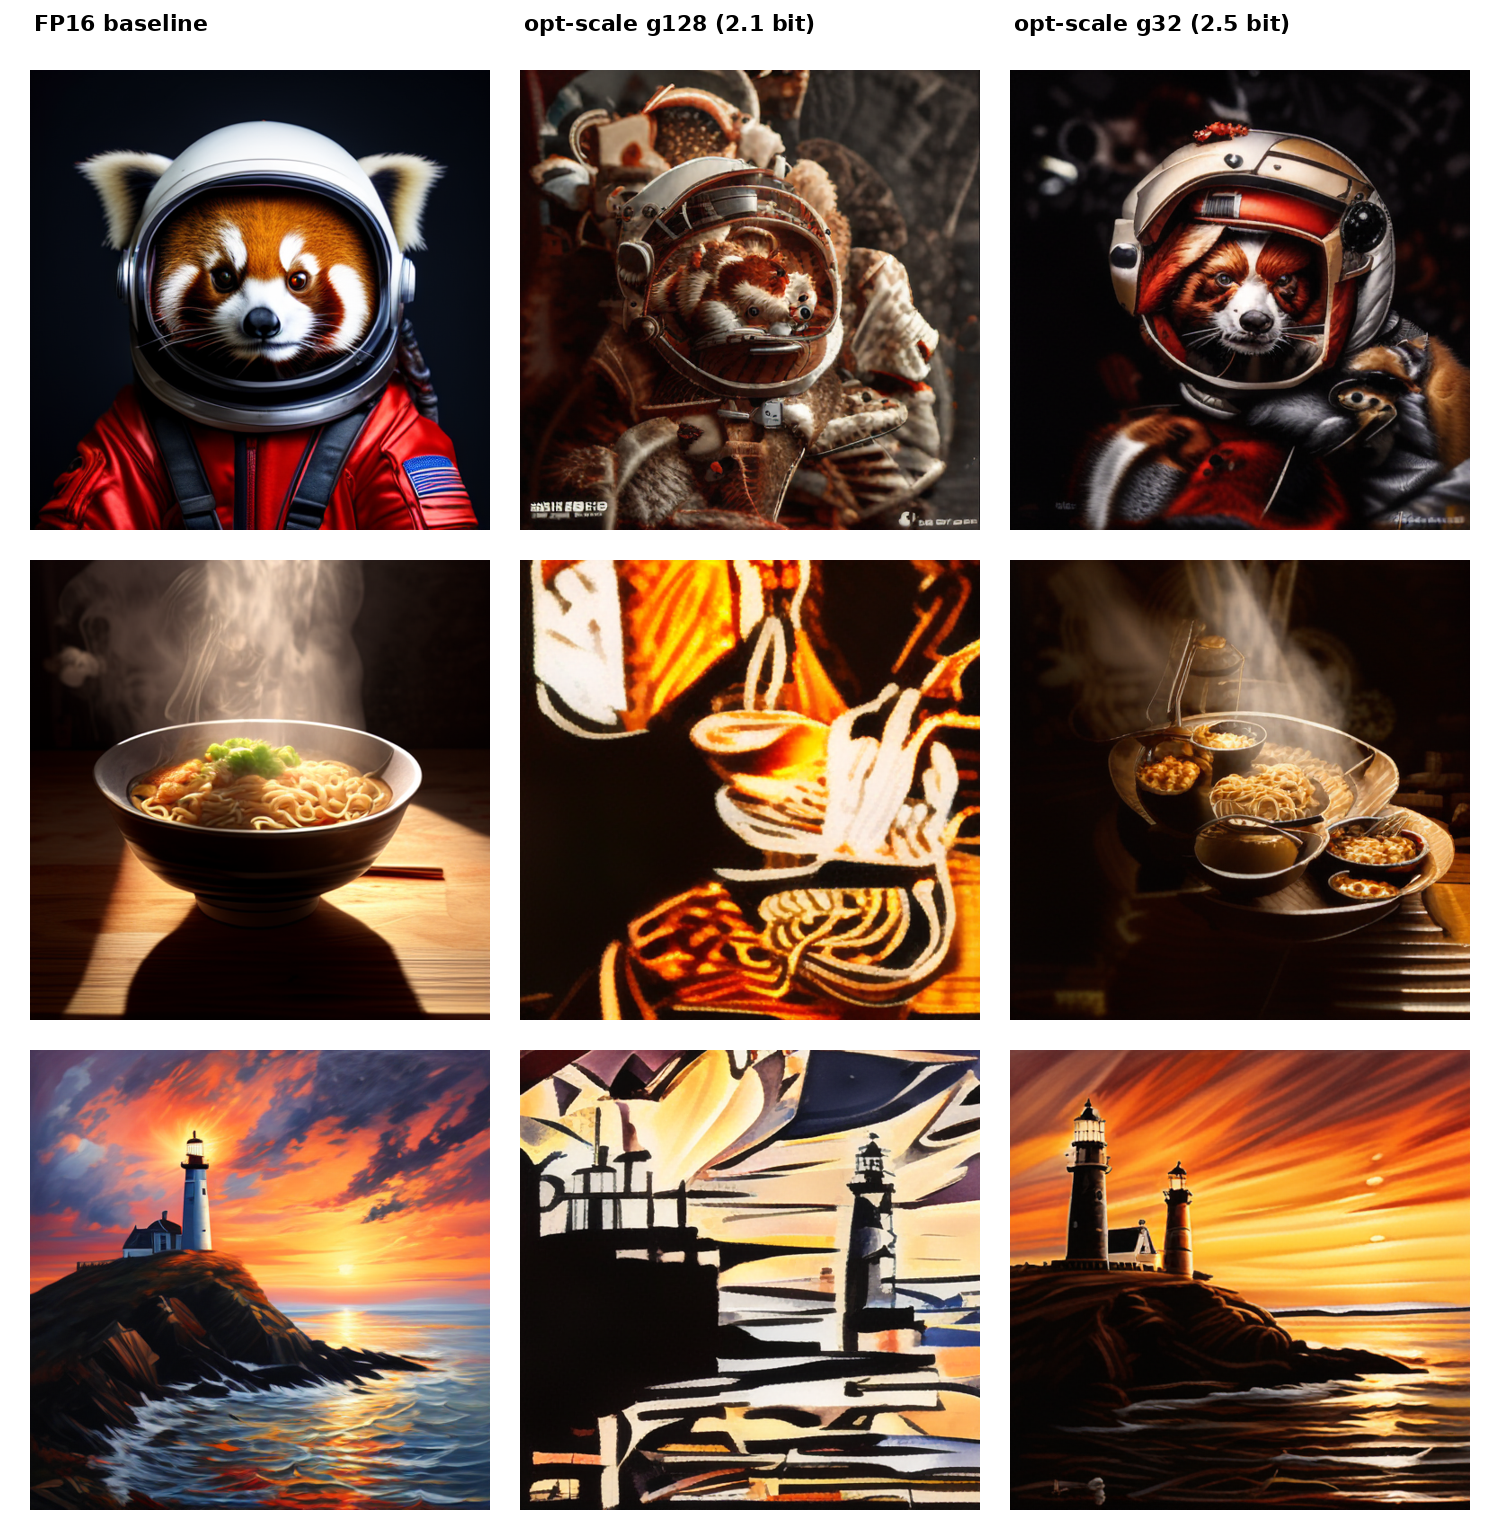
\includegraphics[width=\textwidth]{../assets/compare_final.png}
\caption{Identical prompts and seed. Left: FP16 baseline. Middle: optimal-scale
ternary, $g{=}128$ ($2.1$ bits/wt). Right: $g{=}32$ ($2.5$ bits/wt). Both are
fully data-free with $94.6\%$ of the transformer ternary. Contrast with
\texttt{absmean}/error-feedback, which yield pure noise.}
\end{figure}

\paragraph{Findings.} (1) The scale rule is the dominant lever: swapping
\texttt{absmean} for the optimal scale moves the model from noise to recognizable
images at the same bit-width. (2) Smaller groups help monotonically but modestly.
(3) Error feedback and per-row gain do not help and can hurt. (4) Keeping the six
sensitive layers in higher precision is necessary; protecting additional whole
blocks was not.

\section{Activation-aware ternary: closing the gap to FP16}
The data-free optimal scale minimizes the per-weight error $\|W-W_q\|_F$, but the
network is sensitive to the per-output error $\|(W-W_q)X\|_F$ over its activations
$X$. We close the remaining gap with two activation-aware components, calibrated on
the model's \emph{own generations} (six generic prompts; no external dataset).

\paragraph{GPTQ.} We quantize the columns of $W$ left to right; after quantizing
column $i$ with error $e_i$, we update the not-yet-quantized columns by
$-e_i\,H^{-1}_{i,\,>i}/H^{-1}_{ii}$, where $H=\mathbb{E}[xx^\top]=\tfrac1N\sum xx^\top$
is the input second moment, so the error is steered into directions the
activations tolerate. The per-column quantizer is our group-wise optimal-scale
ternary, with the group scale recomputed from the running weight at each group
boundary.

\paragraph{Incoherence rotation.} Outliers that a single group scale cannot
capture are removed by a shared random orthogonal $R$. For each linear we quantize
in the rotated basis,
\begin{equation}
  y = Wx = (WR^\top)(Rx),\qquad R^\top R = I,
\end{equation}
i.e.\ we store the quantized $WR^\top$ and apply $x\mapsto Rx$ at inference. A
\emph{single} $R$ serves every same-width layer (the identity holds per layer), and
the Hessian rotates analytically, $H\mapsto RHR^\top$, so no re-calibration is
needed. The rotation mixes coordinates so that no weight is an outlier, making each
group near-uniform in magnitude.

\begin{table}[h]
\centering
\begin{tabular}{lcccc}
\toprule
Method & data & eff.\ bits/wt & PSNR vs FP16 $\uparrow$ & outcome\\
\midrule
optimal scale, $g{=}128$            & none & 2.1 & 9.52  & recognizable\\
optimal scale, $g{=}32$             & none & 2.5 & 12.01 & near-baseline\\
\;+ GPTQ, $g{=}128$                 & self & 2.1 & 14.91 & good\\
\;+ GPTQ, $g{=}32$                  & self & 2.5 & 16.53 & strong\\
\textbf{+ GPTQ + rotation}, $g{=}128$ & self & \textbf{2.1} & \textbf{17.01} & \textbf{near-FP16}\\
\bottomrule
\end{tabular}
\caption{Activation-aware ternary at the same $2.1$-bit budget reaches near-FP16
quality. ``self'' = self-calibrated on the model's own generations.}
\end{table}

\begin{figure}[h]
\centering
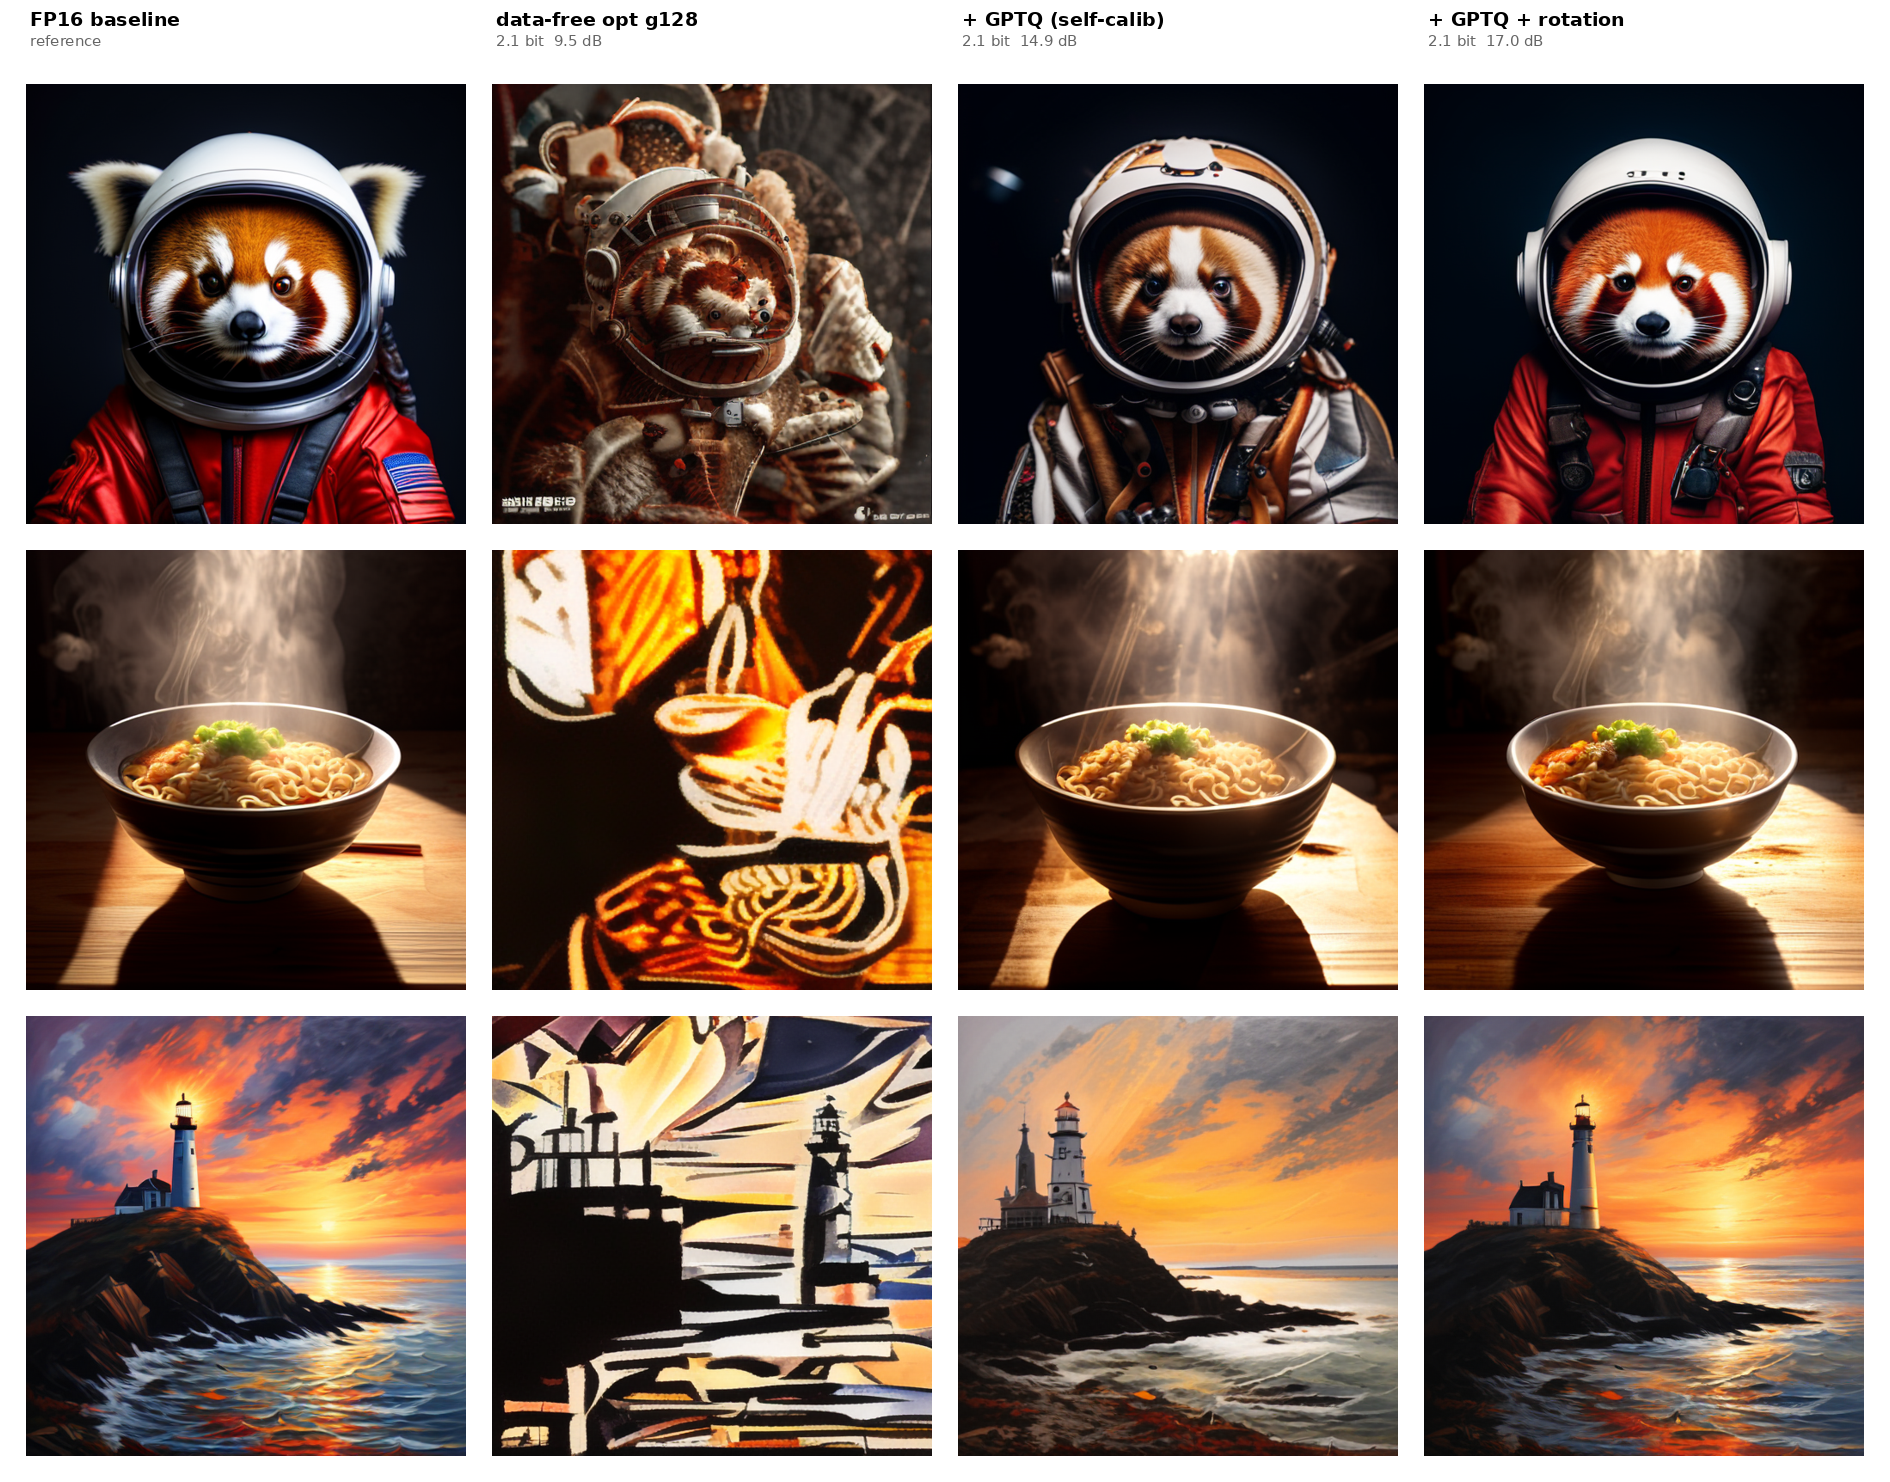
\includegraphics[width=\textwidth]{../assets/compare_activation_aware.png}
\caption{Same $2.1$-bit budget ($g{=}128$, identical seed). Left to right: FP16
baseline; data-free optimal scale ($9.5$\,dB, noise); $+$GPTQ self-calibration
($14.9$\,dB); $+$incoherence rotation ($17.0$\,dB, near-FP16).}
\end{figure}

\section{Data-free self-calibration: the noise+null prior}
GPTQ's only dependence on data is the Hessian $H=\mathbb{E}[xx^\top]$. For a
diffusion model this requires no dataset: the model is built to consume Gaussian
noise, so we capture $H$ by running it on pure noise latents with the null (empty)
prompt---its own unconditional prior. On Sana~1.6B the resulting quantizer is
statistically indistinguishable from one calibrated on real prompts ($16.1$ vs
$15.9$\,dB mean PSNR, visually identical to FP16). The geometry the Hessian
captures is a property of the weights, not of any caption; the model reveals it by
running on its own noise. This removes the last dependence on data and makes the
attention/projection result \emph{fully data-free and train-free}.

\section{The FFN bottleneck: a negative result for scalar ultra-low-bit PTQ}
Ternary attention is near-FP16, but Sana's feed-forward network---a gated
GLU-convolution block---collapses under scalar ultra-low-bit coding regardless of
quantizer. Framing the FFN as a rate--distortion problem and measuring true
symbol-entropy bits (attention fixed at trit $1.71$\,b) gives a frontier: scalar
ternary $0.87$\,b/$10.8$\,dB; uniform 5-symbol $1.73$\,b/$13.3$\,dB; uniform
7-symbol $2.25$\,b/$14.6$\,dB; $4$-bit $3.4$\,b/$16.2$\,dB. Richer alphabets climb
the curve, but every method targeting $\le 2$ bits fails to reach near-FP16: a
Hessian-weighted rank-$32$ residual leaves the FFN at $11$--$15$\,dB; post-hoc
sparse escapes \emph{worsen} GPTQ by disrupting its causal error compensation
($1.2$\,b/$9.0$\,dB); a learned Lloyd--Max codebook \emph{raises} entropy
(distortion-optimal $\neq$ rate-optimal); and a correctly-implemented block
entropy-constrained GPTQ at $1.8$ bits reaches only $8.1$\,dB---worse than the
uniform 5-symbol codebook at the same rate. The mechanism is consistent: a
\emph{global} scalar rate objective drives most coordinates to zero and spends a
few bits on large escapes, destroying the per-group amplitude uniformity the GLU
needs. \textbf{All scalar methods tested fail; the failure mode indicates the
missing information is local and vector-structured} (cross-coordinate amplitude
patterns), pointing to vector quantization or structural channel reduction rather
than any scalar code. We do not claim a formal lower bound.

\section{Clark-Compress: the mixed-precision product}
The practical resolution keeps ternary (GPTQ + rotation) attention and quantizes
the FFN at $4$-bit (data-free). On Sana~1.6B this is near-FP16 ($\sim$16\,dB),
$0.72$\,GB---$4.4\times$ smaller, and $\sim$6$\times$ with trit-packing and FP8/FP6
islands---and fully data-free / train-free. It is the recommended release; the
all-ternary variant ($0.53$\,GB) is degraded and research-only. Reaching $8\times$
at near-FP16 requires either vector-coded FFN (PVQ/TCQ/lattice, which preserves
local amplitude structure by construction) or structural GLU hidden-channel
contraction with closed-form down-projection refit under the same noise prior.

\section{Discussion and limitations}
At ternary precision $\sim\!43\%$ of the weight magnitude is discarded, so outputs
are stylized/posterized rather than pixel-identical; this is intrinsic to the
bit-width, not the method. Our rotation uses a dense random orthogonal matrix for
clarity; a deployment would replace it with a structured fast Hadamard transform
($O(d\log d)$) folded through the residual stream, removing the per-layer matmul
overhead. We focus on a diffusion transformer here; both the data-free optimal
scale and the activation-aware extension apply unchanged to decoder-only language
models.

\section{Conclusion}
Two results frame extreme-low-bit PTQ of a diffusion transformer.
\emph{Positive}: data-free, train-free, near-FP16 quantization is \textbf{solved
for the attention and projection layers} at $1.7$--$2.1$ bits---the closed-form
optimal scale sets the data-free floor, GPTQ with a shared incoherence rotation
sets the quality, and calibrating the Hessian on the model's own noise+null prior
removes the last dependence on data. \emph{Negative}: Sana's GLU-convolution FFN
is the remaining compression bottleneck, and every scalar ultra-low-bit method we
tested fails on it below $\sim$2 bits---the missing information is local and
vector-structured, not scalar. The practical product is mixed-precision
(ternary attention, $4$-bit FFN): data-free, near-FP16, $\sim$4--6$\times$ smaller.
Closing the gap to $8\times$ is a question of vector-coded or structurally-contracted
FFNs, not of better scalar scales.

\begin{thebibliography}{9}
\bibitem{bitnet158} S.~Ma et al. \emph{The Era of 1-bit LLMs: All Large Language
Models are in 1.58 Bits.} arXiv:2402.17764, 2024.
\bibitem{twn} F.~Li, B.~Zhang, B.~Liu. \emph{Ternary Weight Networks.}
arXiv:1605.04711, 2016.
\bibitem{gptq} E.~Frantar, S.~Ashkboos, T.~Hoefler, D.~Alistarh. \emph{GPTQ:
Accurate Post-Training Quantization for Generative Pre-trained Transformers.}
arXiv:2210.17323, 2022.
\bibitem{obq} E.~Frantar, D.~Alistarh. \emph{Optimal Brain Compression.}
arXiv:2208.11580, 2022.
\bibitem{quarot} S.~Ashkboos et al. \emph{QuaRot: Outlier-Free 4-Bit Inference in
Rotated LLMs.} arXiv:2404.00456, 2024.
\bibitem{dfq} M.~Nagel et al. \emph{Data-Free Quantization Through Weight
Equalization and Bias Correction.} arXiv:1906.04721, 2019.
\bibitem{sana} E.~Xie et al. \emph{Sana: Efficient High-Resolution Image Synthesis
with Linear Diffusion Transformers.} arXiv:2410.10629, 2024.
\end{thebibliography}

\end{document}
